\section{Results and Discussion}
System-level simulation was performed with representative AI inference workloads.

\subsection{Standby Power}
Migrating cold data and checkpoints to the FeRAM-backed tier yields more than 30\% reduction in standby power.
This reduction arises from suppressing periodic DRAM refresh for inactive regions.

\subsection{Resume Latency}
FeRAM allows direct restore of checkpoints without full DRAM wake-up.
Resume latency is reduced to the $\mu$s range, enabling near-instant resume after power gating and improving energy efficiency for mobile edge AI.

\subsection{Endurance}
FeRAM endurance of $10^{12}$~writes/year fits within FeRAM capability for checkpoint traffic.

% ===== Fig.2: Access time vs. Retention (pgfplots) =====
\begin{figure}[!t]
\centering
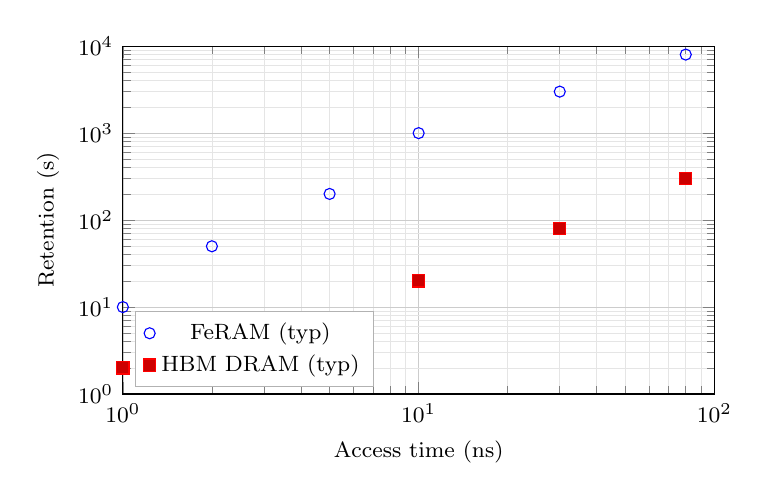
\begin{tikzpicture}
\begin{axis}[
  width=0.75\linewidth, height=6.0cm,
  xlabel={Access time (ns)}, ylabel={Retention (s)},
  xmode=log, ymode=log,
  xmin=1e0, xmax=1e2,
  ymin=1e0, ymax=1e4,
  grid=both,
  tick align=inside,            % ★ 目盛りを内側に
  major grid style={line width=.2pt, draw=black!20},
  minor grid style={line width=.2pt, draw=black!10},
  legend style={at={(0.02,0.02)}, anchor=south west, font=\footnotesize, fill=white, draw=black!30},
  label style={font=\footnotesize},
  tick label style={font=\footnotesize},
]
  % FeRAM (blue circles)
  \addplot+[only marks, mark=o] coordinates
    {(1,10) (2,50) (5,200) (10,1000) (30,3000) (80,8000)};
  \addlegendentry{FeRAM (typ)}

  % HBM DRAM (red squares)
  \addplot+[only marks, mark=square*, mark size=2.2pt] coordinates
    {(1,2) (3,5) (10,20) (30,80) (80,300)};
  \addlegendentry{HBM DRAM (typ)}
\end{axis}
\end{tikzpicture}
\caption{Access time vs. retention. Red squares: HBM; blue circles: FeRAM. Axes restricted to the practical design window ($10^0\!\sim\!10^2$~ns, $10^0\!\sim\!10^4$~s). Legend is kept inside the plot and away from data points.}
\label{fig:retention_vs_access}
\end{figure}
